%\documentclass[twoside,openright,a4paper,11pt,english,draft]{article}
\documentclass[twoside,openright,a4paper,11pt,english]{article}

%\documentclass[twoside,openright,a4paper,11pt,french]{article}
%\documentclass[twoside,openright,a4paper,11pt,french]{book}
\usepackage[utf8]{inputenc}
\usepackage[english]{babel}

% Utilisation de tableaux
\usepackage{tabularx}

\usepackage{subcaption}
\usepackage{wrapfig}

% Utilisation d'url
\usepackage{url}
\urlstyle{sf}

% Utilisation d'images, stockées dans le répertoire ./pics/
\usepackage{graphicx}
\graphicspath{pics/}

% Définition des marges
\usepackage{geometry}
\geometry{%
  left=22mm,%
  right=22mm,%
  top=15mm,%
  bottom=15mm,%
  foot=10mm% 
}

\begin{document}
%XXX add date to title

%%% IRBABOON
\def\j{\emph{Jitsi}}
\def\jvb{\emph{Jitsi-Videobridge}}
\def\bj{\emph{BlueJimp}}
\def\lj{\emph{libjitsi}}
\def\wrtc{\emph{webrtc.org}}
\def\jm{\emph{Jitsi Meet}}


%%% NOOBABRI

% La page de garde
\thispagestyle{empty}

\begin{center}
       \noindent
       \includegraphics[height=2.5cm]{./pics/uds.eps}       
       
       \vfill\vfill

    {\large \textsc{Master 2\\Réseaux Informatiques et Systèmes Embarqués}}

    \bigskip\bigskip

    {\large Presented by}
    %{\large Présenté par}

    \medskip

% Identité de l'auteur
    {\large Boris \textsc{Grozev}}
 
% Contact mail ou téléphone   
    {\small \url{boris@jitsi.org}}

    \vfill\vfill

% Titre du stage
    {\huge \sc
      \begin{center}
		Final Report
      \end{center}}
        \begin{center}
        Media recording for multiparty video conferences based on WebRTC %XXX discuss title
        \end{center}

    \vfill\vfill

    {\large Supervised by:}

\medskip

% Identité de l'encadrant
    {\large Emil \textsc{Ivov}}

% Contact mail ou téléphone
    {\small \url{emcho@jitsi.org}}

\bigskip

    {\large Hosting enterprise:} %XXX that sounds terrible
    %{\large Au sein de}

\medskip

% Structure d'accueil
    {\large \textsc{BlueJimp}}

\vfill\vfill\vfill
           
% Logo de votre structure d'accueil
       %
\includegraphics{./pics/bluejimp2.eps}       
       
\includegraphics[height=2.5cm]{./pics/bluejimp2.eps}

\end{center}


% Page blanche au dos de la page de garde
\newpage
\pagestyle{empty}
\newpage


% La table des matières
\parskip=0pt
\tableofcontents

% Page blanche entre la table des matières et le texte
\newpage
\pagestyle{empty}
\newpage

\pagenumbering{arabic}
\thispagestyle{plain}
\pagestyle{plain}


\begin{abstract}
This document is submitted as part of the requirements for obtaining a masters
degree in informatics at the University of Strasbourg. It describes work done
during a 6-months long internship. A modern video
conferencing application based on WebRTC (\jm)is discussed, and a system for
media recording, which I helped to design and implement, is examined in detail.
The first section serves as an introduction to the work environment for the
internship and the most important technologies discussed later on. The rest 
of the sections examine specific parts of the media recording process.
\end{abstract}




\section{Introduction}
\label{chap:intro}
The first part of this section is about \bj, the company which hosts my internship.
Sections \ref{intro-jitsi} to \ref{intro-jm} are an overview of the
important standards and software products involved in a \jm\ conference.
Finally, section \ref{intro-recording}
defines what we mean by "media recording" and gives a general overview of the
process.




\subsection{\bj}
XXX expand \bj\ section

XXX add dates?



\bj\footnote{\url{https://bluejimp.com}} is a small company which
offers support and development services mainly focused around the
\j\footnote{\url{https://jitsi.org}}
 family of projects. The FLOSS (Free/Libre Open Source Software)
nature of these projects makes for a slightly unusual business model. The
company works with various kinds of customers who all have different use cases
for \j\ and need it adapted to their needs. While \bj\ has no exclusivity
on such adaptations, it is tightly involved in the development of the project
and some of the related technologies and standards. This has helped the company
acquire significant credibility and offer advantageous price/quality ratios.

In addition to orders from customers, \bj\ also often works on internal projects
that aim to enrich \j\ and make it more attractive to both users and
enterprises. 

\bj\ is registered in Strasbourg, but the development team is international,
with people working from different geographic locations. Most communication happens over
the Internet using e-mail, instant messaging and audio/video calls.

My position in \bj\ is that of a software developer. Apart from development, my tasks also 
involve a fair amount of research, experimentation and optimizations. I have
worked on \j\ previously and when my internship began, I was able to quickly
get accustomed to the environment. 




\subsection{The \j\ family}
\label{intro-jitsi}

XXX expand: when jitsi started (sip-communicator)

\j\ is a feature-rich internet communications client.
It is free software, licensed under the LGPL\cite{lgpl}.
The project was started by Emil Ivov in
the University of Strasbourg in 2003, and it was then known as SIP
Communicator. In the beginning
SIP Communicator was only a SIP client, but through the years it has evolved
into a multi-protocol
client (XMPP, AIM, Yahoo! and ICQ are now also supported) with a very wide variety
of features: instant messaging (IM), video calls, desktop streaming,
conferencing (multi-party, both audio and video), cross-protocol calls (SIP to
XMPP), configuration provisioning, media encryption (with SRTP, setup via SDES,
ZRTP or DTLS/SRTP), many audio and video codecs, echo cancellation, session
establishment using ICE, chat sessions encrypted using OTR, file transfers.
Most of the development comes from \bj.

XXX too much features listed?
XXX clean the above paragraph

\j\ is written mostly in Java and runs on a variety of
platforms (Windows, Linux, MacOSX and Android). The various projects comprise a massive codebase--
over 700 000 lines of Java code alone.

A big part of the code which was originally in \j\ is now split into a
separate library-- \emph{libjitsi}. This allows it to be easily reused in other
projects, such as \jvb. The code in \lj\ deals mainly with multimedia-- capture and rendering, transcoding, encryption/decryption and transport over the network of audio and video date. It contains the RTP stack for \j\ (partially implemented in \lj\ itself, partially delegated to FMJ).

\jvb\ is a server-side application which acts as a media
relay and/or mixer. It allows a smart client to organize a conference
using an existing technology (for example, SIP or XMPP/Jingle), outsourcing the bandwidth-intensive task of media relaying to a server. 
The organizing client controls \jvb\ over XMPP\footnote{Although a REST API is also available.}, while the rest of the
participating clients need not be aware that \jvb\ is in use (for example they
can be simple SIP clients). Since the end of 2013 \jvb\ supports ICE and is WebRTC-compatible.

One of the latest additions to the \j\ family is
\jm\footnote{\url{https://jitsi.org/Projects/Jitsi-Meet}}. This is a WebRTC %XXXverify the URL
application, which runs completely within a browser and creates a video
conference using a \jvb\ instance to relay the media.




\subsection{WebRTC}
WebRTC (Web Real-Time Communications) is a set of specifications 
currently in development, that allow browsers which implement them to open
"peer connections" to other browsers. These are direct connections between two
browsers (a webserver is used only to setup the connection), and can be used to
send audio, video or application data. The specifications are open and are meant
to be implemented in the browsers themselves (as opposed to in additional
plug-ins).

WebRTC is divided in two main parts: the JavaScript standard APIs, being defined within
the \emph{WebRTC} working group\cite{webrtc-wg} at W3C,
and the on-the-wire protocols, being defined within
the \emph{RTCWEB} working group\cite{rtcweb-wg} at the IETF.

If implemented, these standards provide web developers with a very powerful tool, which
can be used to create rich real-time multimedia applications very easily. They
also allow for some very interesting and more complicated use-cases.

The specifications are still being developed, but are already at an advanced stage. There is
an open-source implementation of the network protocols, provided by Google with
a BSD-like license. I will refer to this implementation as \emph{webrtc.org}
(which is the domain name of the project). Currently all browsers implementing
WebRTC (Chrome/Chromium and Mozilla Firefox) 
use \emph{webrtc.org} as their base. Because of this, \wrtc\ is very important -- it is
used for all practical compatibility testing, making it the de-facto reference implementation.




\subsection{XMPP and Jingle}
Extensible Messaging and Presence Protocol (XMPP)\cite{rfc6120} is a mature,
XML-based protocol which allows endpoints
to exchange messages in near real-time. The core XMPP protocol only covers instant messaging (that is the exchange of
text messages meant to be read by humans), but there are a variety of extensions that allow the protocol
to cover a wide range of use cases. Many such extensions are published as XMPP Extension Protocols (XEPs), and there are XEPs which allow for
group chats, user avatars, file transfers, account registration, transporting
XMPP over HTTP, discovering node capabilities, management of  wireless sensors (provisioning, control, data collection),
and, most relevant here, internet telephony.

\emph{Jingle}\cite{jingle166, jingle167} 
is a signalling protocol, serving a purpose similar to that of SIP: it uses an
offer-answer model to setup an RTP session. Many of the
protocols often used with SIP, such as ICE\cite{ice}, ZRTP, DTLS-SRTP, and
RFC4575 can also be used with \emph{Jingle}. Mappings
have been defined between the two\cite{stoxmedia}, which allow gateways or rich
clients to organize cross-protocol calls.

\begin{wrapfigure}{r}{0.4\textwidth}
   \centering
        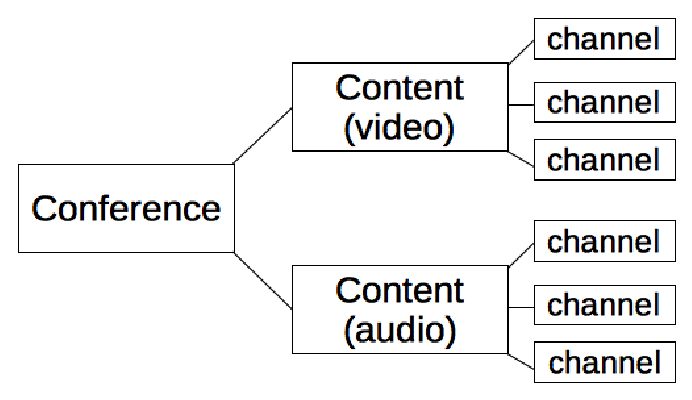
\includegraphics[width=0.35\textwidth]{./pics/colibri-conf.eps}
        \caption{A COLIBRI conference.}
   \label{colibri-conf}
\end{wrapfigure}

COnferencing with LIghtweight BRIdging (COLIBRI\cite{colibri}) is an extension
developed mostly in \bj\ for use with \jvb. It provides a way for a client to control a multimedia
relay or mixer, such as \jvb. It works with the concept of a \emph{conference}, which contains
\emph{channels}, separated in different \emph{contents} (see fig.\ref{colibri-conf}). A
client requests the creation of a \emph{conference} with a specified number of
channels. The mixer allocates local sockets for each \emph{channel} and
provides their addresses to the client. The client can then use these transport
addresses as its own to establish, for example, a \emph{Jingle} call. 
Instead of just allocating local sockets, the ICE protocol can be used, in
which case the mixer provides a list of ICE candidates for each \emph{channel}.
The protocol works with a natural XML representation of a \emph{conference}.
After the \emph{conference} is established, the client can add or remove channels
from it, or change the parameters (such as the direction in which
media is allowed to flow) of an existing \emph{channel}.





\subsection{A \jm\ conference}
\label{intro-jm}
\jm\ uses the above-mentioned technologies to create a multi-party video conference.
The endpoints of the conference are simply WebRTC-enabled
browsers\footnote{Although at the present time only Chrome/Chromium and Opera are
supported.} running the actual \jm\ application. They all connect to an XMPP
server and join a Multi-User Chat (MUC) chatroom. One of the participants (the
first one to enter the chatroom) assumes the role of organizer (or focus).

The focus creates a COLIBRI conference on a \jvb\ instance $jvb$, and allocates
two COLIBRI channels for each participant (one for audio, and one for video).
Then, it initiates a separate \emph{Jingle} session with
each participant, using the
transport information (i. e. the list of ICE candidates) obtained from $jvb$
instead of its own. When the participants accept the Jingle sessions, they in
effect perform ICE and establish direct RTP sessions with $jvb$.

The resulting connections are depicted in Figures \ref{jitmeet-sig} and \ref{jitmeet-med}.


XXX update figures
\begin{figure}[h]
   \centering
        \begin{subfigure}[t]{0.4\textwidth}
            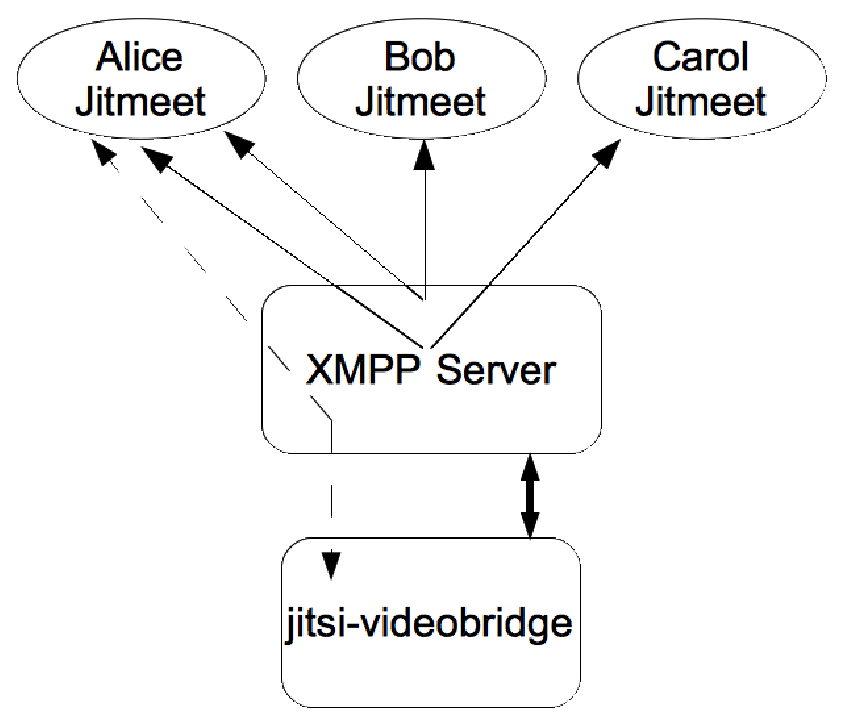
\includegraphics[height=5.5cm]{./pics/jm-sig.eps}
            \caption{Signalling connections in a \jm\ conference.
                The solid lines are XMPP/Jingle sessions, the dashed line
                is XMPP/COLIBRI. The thick line is an XMPP Component Connection.}
            \label{jitmeet-sig}
        \end{subfigure}
        \quad
        \quad
        \quad
        \begin{subfigure}[t]{0.4\textwidth}
            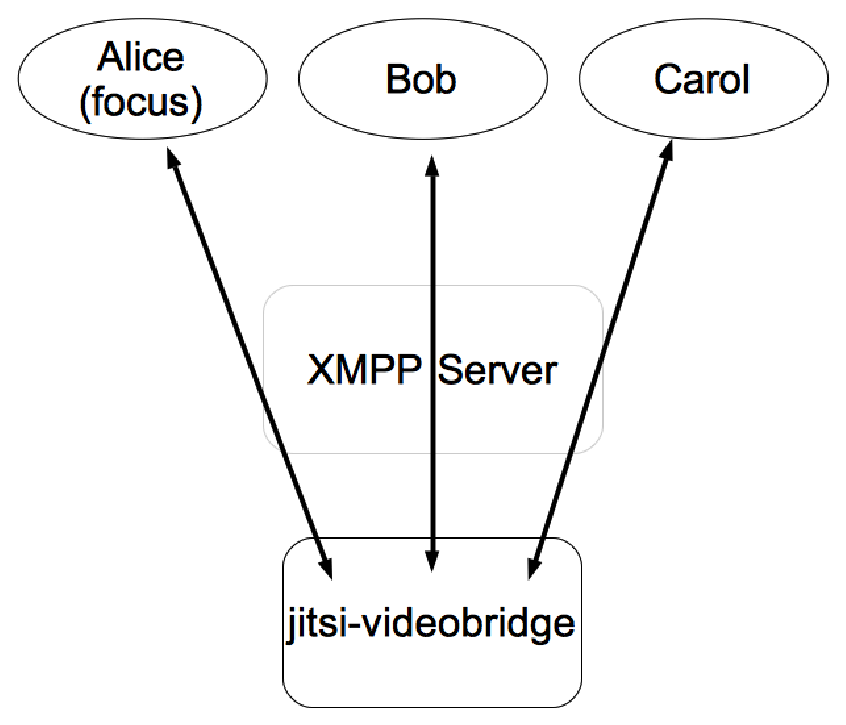
\includegraphics[height=5.5cm]{./pics/jm-med.eps}
            \caption{Media connections in a \jm\ conference. The
                lines represent RTP/RTCP sessions.}
            \label{jitmeet-med}
        \end{subfigure}
\end{figure}


\smallskip
On the user-interface end, \jm\ aims to make it as easy as possible for a
person to enter or organize a conference. 
Entering a conference is accomplished by simply opening a URL such as \emph{https://meet.jit.si/ConferenceID} 
(where \emph{ConferenceID} can be chosen by the user). If \emph{ConferenceID}
doesn't exists, it is automatically created and
the user assumes the role of focus, inviting anyone who enters later on. If
\emph{ConferenceID} exists,
the user joins it (possibly after entering a password for the conference).

When in a conference, the interface has two main elements: one big video
(taking all available space) and, overlayed on top of it,
scaled down versions of the videos of all other participants. Figure
\ref{jm-ss} is a screenshot from the actual application. The video shown in
full changes, according to who is currently speaking.

\begin{figure}[h]
    \includegraphics[width=1\textwidth]{./pics/jm-ss.eps}
    \label{jm-ss}
    \caption{A screen capture from a \jm\ conference.}
\end{figure}

XXX able to install your own \jm



\subsection{Recording}
\label{intro-recording}
By recording a multimedia conference in general we mean the following: all the
audio and video involved in the conference
is saved to disk in some format, in a way which allows the whole conference to
be played back later on.

\medskip
In our specific case, the recording of a conference has three main parts:
\begin{itemize}
\item{Recording media}
\item{Recording metadata}
\item{Post-processing}
\end{itemize}

Recording of the media is the process in which the audio and video RTP streams
in the conference are converted to a convenient format and saved to disk. There
are many different ways in which this can be done. Our final solution (and some
of the ideas that didn't work) are discussed in detail in
sections \ref{recording-video} and \ref{recording-audio}.

Recording of metadata means saving additional information (apart from the media
itself) which is necessary to play back the conference later. This includes
timing information, participant names and changes of the active speaker. There
is a detailed discussion of the
metadata that we use in section \ref{recording-metadata}.

Post-processing in our case means taking all the recorded data and producing a
single file with one audio track and one video track. The specifics depend on
configuration, but
generally all audio is mixed together, and the videos are combined in a way to
resemble the \jm\ interface. Appendix \ref{jipopro} discusses the
post-processing application.


\paragraph*{Where does recording happen?}
As can be seen in figure \ref{jitmeet-med}, in a \jm\ conference both \jvb\ and
all the participants have access to the RTP streams, and so could potentially
perform recording.

Since the participating clients are running an application within their
browser, if we want one of them to do recording, we would need modifications to
the browsers (which is undesirable). To avoid this, a "fake participant" can
be added to the conference, which does not not actually participate in the conference
(does not send audio or video), and does not run in a browser.

Recording directly on \jvb\ is more straightforward, so our initial
implementation was focused on that. However, most of the code resides in \lj, allowing
it to be easily reused.

Li Shunyang, a student from Peking University, is currently working, under the
Google Summer of Code program, on a recording
application\footnote{https://github.com/jitsi/jirecon} which uses
the "fake participant" approach.




\section{The WebRTC transport layer}
This section is about transporting media in webrtc. Uses ICE to establish a
UDP (or TCP) connection, then makes a DTLS/SRTP (in the case of media) stream.
\subsection{RED}
\subsection{ULPFEC}
ULPFEC (stupid idea with re-writing sequence numbers. why adding FEC arbitrary to the stream makes it impossible to decode correctly. what webrtc does. how we handle it by just removing my stupid code). Diagrams
diagrams

\bigskip
The peer connections between browsers use the Real-time Transport Protocol (RTP\cite{rtp}), and WebRTC mandates the use of
Interactive Connectivity Establishment (ICE\cite{ice}) for session establishment.

WebRTC defines two mandatory to implement audio codecs: G.711\cite{g711} and
Opus\cite{opus, opusrtp}. This guarantees that any two compliant browsers can establish
an audio session. For video, however, the situation is not so simple, with no
decision having yet been made on a mandatory to implement codec. Google's VP8\cite{vp8}
codec is the one implemented in \emph{webrtc.org} and is therefore the de-facto
standard at the moment.


\subsection{Retransmissions}

\section{Recording video}
\label{recording-video}
\jm\ conferences use the VP8 codec for video.
VP8 stuff

When we were choosing a container format for the video recordings, we considered three options.
The first was to use the very simple and limited \emph{ivf} format. This is a video-only format
that comes from the \emph{libvpx} test-suite and example applications. The second option was to use \emph{webm}.
ivf, webm, our own format.
Webm stuff

How do we timestamp frames -- easy compared to audio

diagraam: transformers -> jitter buffer -> depacketizer -> webmdatasink

Comparison with the WebRTC stack?

Note: no decoding/encoding.

Jitter buffer stuff goes here

Partial vp8 frames -- nothing done so far, only discussions

Requesting keyframes

\section{Recording audio}
\label{recording-audio}
We tried mixing streams live -- difficult to sync

Decided to record them separately

Still problems with sync: lost packets cause "holes" and in a long recording video starts to progressively lag more and more.
Needed to add silence: allows for perfect sync (up to a sample)

Problem with too much silence (e.g when someone unmutes). Restarting streams when too much silence detected

We reencode to mp3 (because we have mp3 support ready). We want to do ogg/opus, and avoid decoding and encoding altogether. Problem: FEC

diagram:
transformers -> jb -> decoder -> silence -> encoder + datasink

FEC (opus): how it works. when we reencode audio, we take advantage of it automatically (already implemented in the decoder).

diagram: how would it look with ogg/opus
\section{Recording metadata}
\label{recording-metadata}
What is the metadata used for. Sample JSON

Important information: filenames and timestamps

speaker changed events


\section{Synchronization}
Purpose: audio and video from a single participant need to be perfectly synchronized. Need to use the timestamps from the source, because of network jitter. 

How it works: RTCP sender reports and the info they contain.

My lovely Synchronizer class. Diagrams (I have some on paper, also sync.pdf somewhere)

\section{Dominant speaker identification}
\label{dsd}
Dominant speaker identification (DSI) refers to the process of continuously analysing a set of audio streams
(which are assumed to contain human voice) and keeping track of the one which
comes from the person currently speaking (or the person currently speaking "the
most"). Obviously the problem does not have a single solution, and so it is hard
to measure objectively how well a system performs. A good description of the
general problem and a proposed solution is available in \cite{volfin2012}. 

In a \jm\ conference there are two use-cases for DSI: for use "live" in a
conference and for recording. 
For "live" use, the purpose is to have the client interface change during a
conference, according to who is the dominant speaker (i.e. the video shown in
full changes when the dominant speaker changes). In this case DSI is performed
on \jvb, which uses WebRTC data channels to notify the clients of the change.

For use in recording, the purpose is for the post-processing application to
take into account the dominant speaker when combining the videos (in general,
it follows the \jm\ interface and renders the dominant speaker in full size).
In this case, DSI is performed on the recording application, and changes of
the dominant speaker are saved as metadata.

\paragraph*{Implementation}
My task was to design and implement an API and a simple, non-optimized
algorithm , which we could later improve upon. 

I came up with a very simplified scheme, implemented it and tweaked its parameters until it seemed to
work well in a conversation with two people. It only takes into account the
audio levels (that is, the loudness of the sound) of the different streams. It
works like this:

At all times one stream is considered active, while the rest are considered
'competing'. All streams have an associated score. When new audio levels are
measured for a stream its score is recomputed,
and the scores of all streams are examined in order to determine if one of
the competing streams should replace the then active stream.

In order to be 'eligible' to replace the active stream, a competing stream has to:
\begin{enumerate}
    \item Have a score at least $C$ times as much as the score of the currently active stream.
    \item Have score at least MIN\_SCORE.
    \item Have been active in the last MIN\_ACTIVE milliseconds.
\end{enumerate}

The first rule helps to avoid often changing the active when there are two
streams with similar levels. The second prevents the active speaker from being
changed during a pause of his speach, while no one else is speaking either (but
someone else generates higher levels during "silence" than the speaker). The
third is to make sure that when participants leave a conference, they aren't
mistakenly chosen as active (this is due to implementation details)

The values for the parameters are very dependent on the exact rules for scoring.
I chose the values based on a few uncontrolled experiments we performed. I used
MIN\_ACTIVE $= 1000$ and $C = 1.15$ (MIN\_SCORE is too arbitrary to deserve mention).

Scores are computed as follows: $C_{recent} * avg(0, N_1) + C_{older} * avg(N_1, N_2)$
where $avg(X_1, X_2)$ is the average audio level for the interval $[now-X_2,
now-X_1)$ (in milliseconds). 

Currently the values of the parameters are: $C_{recent} = 2, C_{older} = 1, N_1 = 250, N_2 = 1250$.


\bigskip
We found that this solution works sufficiently well, at least for the purposes
of testing recording and post-processing. One problem that we face is when
one of the participants is generating constant noise (caused for example by a
spinning fan near the microphone). In this case the algorithm tends to select this participant,
even if they are not speaking. One suggestion for a fix is to measure the
variance of the sound levels for a participant, and penalize the score if the
variance is low. This depends on the assumption that a person speaking would
produce sound with varying loudness (and that this variation can be detected
with the 20ms resolution that we use). However, we have not yet tried to solve
this problem.

Lyubomir Marinov has now taken over this task, and has implemented an improved algorithm that more closely resembles the
one proposed in \cite{volfin2012}. However, his implementation still relies on
"audio levels" and not on other analysis of the audio samples. This offers a significant advantage
in our use case, because this information (the "audio level" for a particular RTP packet) is already
calculated by the sending client, and is included in the RTP packet in the format specified in RFC6464\cite{rfc6464}.
This allows \jvb\ to do DSI very cheaply, without the need to decode the received audio streams.




\section{future work}
RTX, recording in ogg/opus, postprocessing, jitter buffers?


XXX TODO: support for RTCPCompoundPackets: does it fitsomewhere above?

XXX might scratch "future work" altogether?

\section{Conclusion}
XXX Crap, I almost forgot about this!

\appendix
\section{Post-processing}
\label{jipopro}
Jipopro

\end{document}

\subsection{Recording a conference on \jvb}
The main project on which I have worked since the beginning of the internship
is allowing for a multimedia conference to be recorded by \jvb. Most of the
specific tasks that follow are required by this general goal, and reaching it
is their primary motivation.

For each conference that \jvb\ manages, it receives multiple RTP streams
(generally one audio and one video stream from each participant). For the video
streams it acts as an RTP Translator (as defined in Section 7 in \cite{rtp}). That is, it just forwards RTP packets (re-encrypting them, if necessary), without considering their payload.
For audio streams it can run either as a Translator or as a Mixer (again
defined in Section 7 in \cite{rtp}), depending on runtime configuration. 
When it runs as a Mixer, it decodes all received audio
streams, creates a different "mix" for each participant, encodes that mix and sends
it (and only it) to that participant.

Relaying audio consumes more bandwidth, but is less computationally intensive for \jvb.

\medskip
%XXX add picture?

\subsection{Improve the VP8 implementation}
VP8 is a video compression format, defined in RFC6386\cite{vp8} (with the RTP payload format defined in \cite{vp8rtp}). It is one of the two main video codecs
considered for WebRTC and
the only video codec implemented in
\emph{webrtc.org}. Having a \emph{webrtc.org}-compatible implementation of VP8
is necessary in order to make recordings. Additionally, it can be used later to
connect the desktop \j\ client to a WebRTC endpoint (for example, add it to a
\jm\ conference).


\j\ has a rudimentary VP8 implementation\footnote{Which I added in early
2013.}, but it is not compatible with the specification (and not compatible
with \emph{webrtc.org}). It has four parts: a Decoder, Encoder, Packetizer and
DePacketizer. The first two deal with converting a VP8 compressed frame into
an uncompressed image and vice-versa (using \emph{libvpx}\footnote{\url{http://www.webmproject.org/code/}}). The Packetizer splits a VP8 frame into
RTP packets, and the DePacketizer collects RTP packets and constructs a VP8
compressed frame.

I reviewed the existing code and we decided to only fix the DePacketizer at
this point. This is enough for the purposes of recording and should make our
implementation compatible with \emph{webrtc.org}.

I also reviewed the \emph{webrtc.org} code to see if we can reuse something. I found that the
only thing which we can directly reuse is the Packetizer. For the DePacketizer,
it is easier to modify our existing one.


The actual implementation of the new DePacketizer took only two or three days and there
weren't any difficulties. 

Later on we might continue this work by improving the other parts. Notably, we
can add support for Packet Loss Concealment (PLC), retransmissions (RTX) and
other quality improvement techniques.

\subsection{RED}
RFC2198\cite{red} defines an RTP payload-type that allows the encapsulation of one or more "virtual" RTP packets in a single RTP packet. It is intended to be used with redundancy data.

In \wrtc, RED is used for video streams. Its use is negotiated as a regular media format and it does not have a static payload-type number, so a dynamic number is assigned during negotiation. In the case of a
\jm\ conference, it is negotiated between the clients and \jvb\ has no way of
affecting its use or its payload-type number, because it does not actively participate in the
offer/answer procedure. This means that in order to record video, \jvb\ must understand RED.

My task was to implement RED in \lj. We decided that the best way to do it is to use
a PacketTransformer. In \lj, when an RTP packet is received from the network,
it goes through a chain of elements called PacketTransformers, before being
passed on to the media stack. Example transformations include decrypting SRTP
packets, stripping certain RTP header extensions, and re-writing the
payload-type numbers. See figure \ref{transform}.

PacketTransformers operate on single packets: they take a single packet as
input and produce one as output. Since RED can contain multiple "virtual"
packets, I needed to modify the infrastructure, so that PacketTransformers take
as input a set of packets and output a set of packets.

This part was tricky, because I had to make sure that my changes didn't brake
existing code. After that, the RED implementation was simple.

\begin{figure}[h]
   \centering
        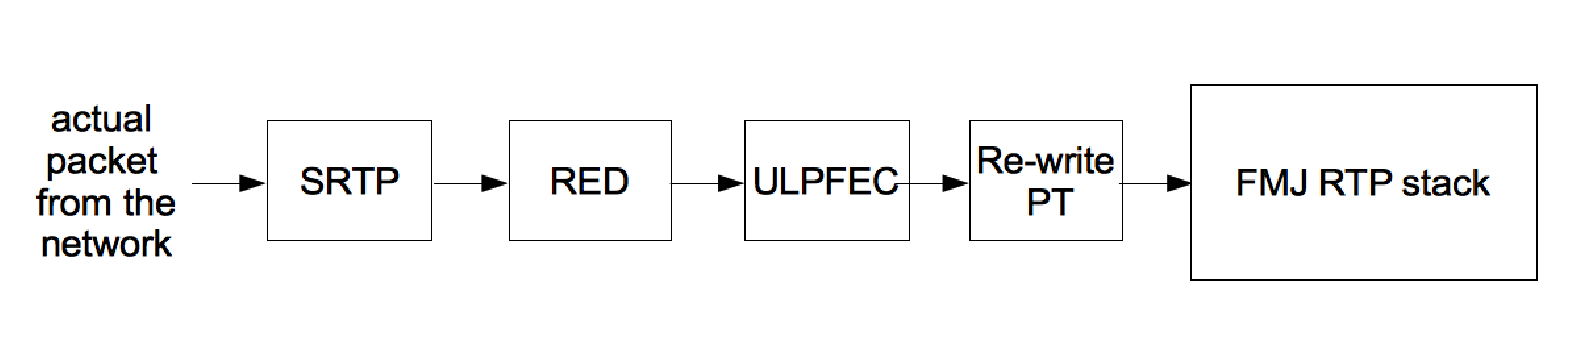
\includegraphics[width=0.9\textwidth]{./pics/transform.eps}
        \caption{Chain of PacketTransformers in \lj.}
   \label{transform}
\end{figure}

%difficulties
\subsection{Uneven Level Protection Forward Error Correction}
In general, Forward Error Correction (FEC) refers to a mechanism which allows
lost data to be recovered without retransmission. It involves sending redundant
data, in one way or another.

RFC5109\cite{ulpfec} defines a specific RTP payload-type for
redundant data called Uneven Level Protection FEC (ULPFEC). It is generic, meaning that it can be used with any media payload-type
(audio or video, no matter what the codec is). 

In \emph{webrtc.org},
ULPFEC is used with video\footnote{For audio, Opus' own FEC scheme which works differently than ULPFEC is used (and it is already supported in \lj).},
and while not strictly mandatory for our video-recording (as opposed to RED), it is important because by decreasing the number of irretrievably lost packets, it will improve the quality of the recordings.
My task was to implement support for ULPFEC in \lj.

ULPFEC (in the rest of the section I will refer to it as simply FEC) is applied to
an RTP stream (the "media stream", with "media packets")
and adds additional packets to it ("FEC packets"). The basic idea is simple --
take a set $S$ of a few media packets and apply a parity operation (XOR) on it,
resulting in a FEC packet $f$. If any one of the packets in $S$ is lost,
the receiver can use the rest of the packets in $S$ together with $f$ to reconstruct the
lost packet\footnote{This is similar to how RAID5 works}. 

Along with the parity data, a FEC packet contains two fields which are used to
describe the set $S$ from which it was constructed: a "sequence number base"
field, and a bitmap field that describes the sequence numbers of the packets in
$S$ using the base. The packet $f$ is said to "protect" the packets in $S$. This scheme 
allows FEC to work without any additional
signalling (apart from the payload-type number negotiated during session
initialization). 

\medskip
We decided to implement FEC as another PacketTransformer. This is how it works:

Two buffers of packets are kept: $bMedia$ and $bFEC$. With every FEC packet $f$
is associated the number $numMissing(f)$ of media packets protected by $f$
which have not been received.

On reception of a media packet, the values $numMissing(f)$ are recalculated for
all $f$ in the $bFEC$ buffer. Then, for all $f$ in $bFEC$: if $(numMissing(f)
== 0)$, then $f$ is removed from $bFEC$. If $numMissing(f) > 1$, then do
nothing. If $numMissing(f) == 1$, use $f$ and $bMedia$ to reconstruct a media
packet and remove $f$ from $bFEC$.

On reception of a FEC packet $f$, $numMissing(f)$ is calculated, and the same
as above is done according to its value.

$bFEC$ is limited to a small size and if a new FEC packet arrives while it is
full, the oldest FEC packet is dropped. This prevents "stale" FEC packets (for
which $numMissing$ will always be $>1$, because more than one of their
protected packets have been lost) to accumulate and cause needless computation.

FEC packets are never passed on to the rest of the application.

\medskip
One complication arises because of the way \lj\ is structured. The code which
calculates packet loss and sends RTCP reports resides in FMJ (that is, later in the chain than the FEC transformer, see Figure \ref{transform}).
So if we just drop the FEC packets, they will be incorrectly considered lost.
For this purpose we chose to keep track of the number of FEC packets received,
and re-write the media packets' sequence numbers accordingly. See Figure \ref{fec-seqs} for an illustration.

\begin{figure}[h]
   \centering
        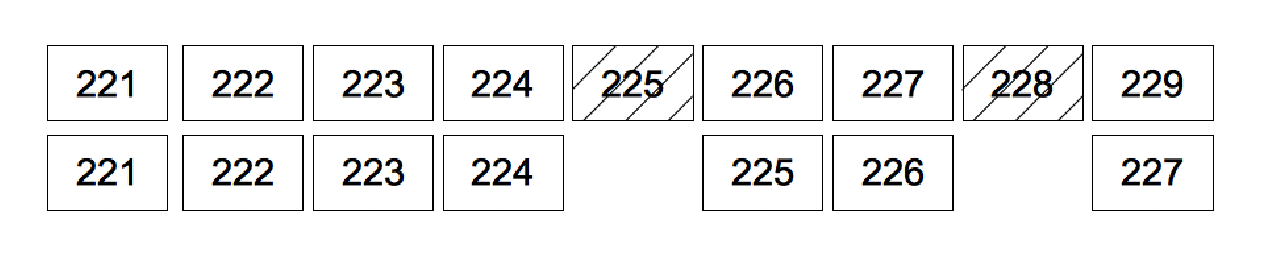
\includegraphics[width=0.9\textwidth]{./pics/fec-seqs.eps}
        \caption{Re-writing sequence numbers after removal of FEC packets. The marked packets are FEC. The line above shows the sequence numbers before FEC is removed, the line below-- after.}
   \label{fec-seqs}
\end{figure}

\subsection{Recording RTP streams}
This task is about the actual recording to disk of the received RTP streams.

\paragraph*{Audio streams}
For audio streams we decided to do the mixing in the application (as opposed to
saving each stream to a separate file and mixing them later). This is because
\lj\ already has all the necessary components. 

\paragraph*{Video streams}
We decided to handle video streams one-by-one. For the moment we support only
VP8, and for that reason we decided to use the \emph{webm} container format. Also, this well-known format allows us
to later use other already available tools, such as \emph{ffmpeg}, for post-processing.

We found an existing library which can write files in \emph{webm} format and I adapted it
to our needs.

\paragraph*{Requesting keyframes}
VP8 has two types of frames: I-frames (keyframes) and P-frames. In order to start working, a decoder
needs to be initialized with a keyframe. Therefore, we want the recorded webm files to start with a keyframe.

Because keyframes are rarely sent, and because we want to be able to start
recording a conference at any time, we need a way to trigger the generation of a
keyframe. One way to do this, which is supported by \wrtc, is by the use of
RTCP Full-Intra Request (FIR) feedback messages (defined in
RFC5104\cite{rfc5104}, section 3.5.1).

The difficulty we faced is that FIR messages contain an "SSRC of packer sender" field, and
\wrtc\ clients only accept messages from SSRCs that they know about (that is,
that have been specifically added via signalling). One possible solution was
for the recorder to spoof the SSRC of another participant. However we opted for
a proper solution in which \jvb\ announces an SSRC of its own in COLIBRI, and
that SSRC is used when sending FIR messages.

\paragraph*{Metadata}
After the audio and video streams have been recorded as described above, we are left
with one audio file and a set of video files. In order to combine them together we need
one important piece of information: timing.

We decided that we are going to create a separate file that contains metadata about the
recordings and that it will contain a list of "events",
which signify for the beginning or end of a recording or possibly something
else. We chose a JSON format, and these are a few examples of such events:

\begin{verbatim}
{
"ssrc" : 3360910907,
"filename" : "3360910907.webm",
"aspectRatio" : "16_9",
"type" : "RECORDING_STARTED",
"instant" : 1395767658389,
"mediaType" : "video"
}

{
"ssrc" : -1,
"filename" : "audio.mp3",
"type" : "RECORDING_ENDED",
"instant" : 1395767704521,
"mediaType" : "audio"
}

{
"ssrc" : 500778727,
"audioSsrc" : 1277672956,
"type" : "SPEAKER_CHANGED",
"instant" : 1395767658527,
"mediaType" : "video"
}
\end{verbatim}

The meaning of the first two should be clear-- they indicate that a certain
file begins at a certain moment in time. 
The third one indicates that the dominant speaker (described in more detail in
the section) has changed. The value for "ssrc" is the SSRC of the video stream
of the new dominant speaker.

The current implementation uses the system time at the moment of reception of
the first recorded RTP packet for RECORDING\_STARTED events. This is not reliable
and sometimes leads to the audio and video not being synchronized in the final recording.

One of my next tasks is to improve this, by using the timing information
contained in RTCP.

\section{Future work}
My next task is to improve the timing of the recording events we generate, so
that audio and video would be synchronised. The most accurate way of achieving
this would be to rely on timing information from RTCP messages and the RTP
timestamps.

Next I will focus on adding support for VP8 PLC (Packet Loss Concealment) to be used with
recording. PLC is a \emph{libvpx} feature which allows the decoder to decode
frames, even when parts of them are missing. Since while recording we do not
have a live decoder (and adding one would be undesirable, because it would make
the process very CPU-intensive), we will need to save files in a
format which supports additional information about frames, which we can later
use in an external application in order to decode partial frames. 

I will also be implementing more advanced reliability mechanisms such as RTP 
retransmissions (RTX)\cite{rfc4588}.
 
Then, once recording quality is satisfactory I will proceed with an improved
scheme for dominant speaker detection. 
  
I will also be attempting to turn the video recorder into a standalone
application in order to improve the scalability of the entire solution.


\section{Conclusion}
During the internship so far, I have studied in detail how the media transport layers in
a \jm\ conference work, and have implemented support for some of the protocols in \lj. I have also
helped with the design and implemented significant parts of a system which allows the recording of the
audio and video in a \jm\ conference.

During the rest of the internship I hope to improve the existing code and to study in more depth
the problem of dominant speaker detection.
\clearpage
\bibliographystyle{plain}
\bibliography{rapport-stage}

\end{document}

